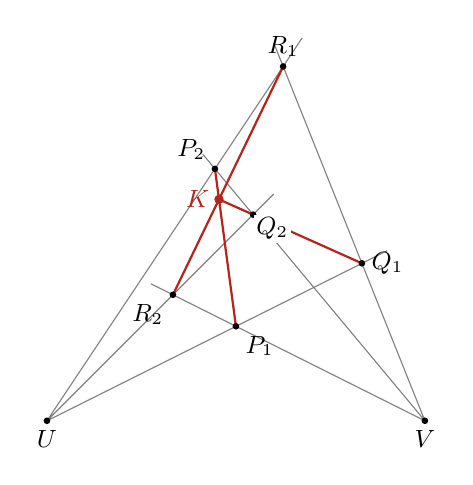
\begin{tikzpicture}[x=1.2cm,y=1.2cm,font=\small]
\coordinate (U) at (-2,0); \coordinate (V) at (2,0);
\coordinate (P1) at (0,1); \coordinate (P2) at ({-2/9},{8/3});
\coordinate (Q1) at ({4/3},{5/3}); \coordinate (Q2) at ({2/11},{24/11});
\coordinate (R1) at (.5,3.75); \coordinate (R2) at ({-2/3},{4/3});
\coordinate (K) at ({-12/67},{157/67});
\draw[gray] (U)--(1.6,1.8) (U)--(.7,4.05) (U)--(.4,2.4);
\draw[gray] (V)--(-.35,2.82) (V)--(-.9,1.45) (V)--(.4,4);
\draw[BrickRed,thick] (P1)--(P2) (Q1)--(K) (R1)--(R2);
\foreach \p in {U,V,P1,P2,Q1,Q2,R1,R2} \fill (\p) circle (1.2pt);
\fill[BrickRed] (K) circle (1.7pt);
\node[below] at (U) {$U$}; \node[below] at (V) {$V$};
\node[below right] at (P1) {$P_1$}; \node[above left] at (P2) {$P_2$};
\node[right] at (Q1) {$Q_1$}; \node[below right,fill=white,inner sep=1pt] at (Q2) {$Q_2$};
\node[above] at (R1) {$R_1$}; \node[below left] at (R2) {$R_2$};
\node[left,BrickRed] at (K) {$K$};
\end{tikzpicture}
